\documentclass[12pt,a4paper]{report}
\usepackage{setspace} 
\usepackage{tocloft} 
\usepackage{graphicx}
\usepackage{ulem}
\usepackage{titling}
\usepackage{amsmath}
\usepackage{geometry}
\usepackage{setspace}
\usepackage{ragged2e}
\usepackage{listings}
\usepackage{xcolor}
\usepackage{float}

\geometry{left=3.5cm, top=2.5cm, right=1.25cm, bottom=1.25cm}

\doublespacing

% Dart syntax highlighting
\renewcommand{\lstlistingname}{Code}
\lstdefinelanguage{Dart}{
    keywords={class, this, void, if, else, for, while, return, async, await, Future, List, Map, Set, try, catch, finally, int, String, var, const, final, static, print, new, null},
    keywordstyle=\color{blue}\bfseries,
    ndkeywords={bool, true, false, null},
    ndkeywordstyle=\color{magenta}\bfseries,
    comment=[l]{//},
    commentstyle=\color{gray}\ttfamily,
    stringstyle=\color{orange}\ttfamily,
    morestring=[b]',
    morestring=[b]",
    tabsize=2,
    showspaces=false,
    showstringspaces=false
}

% Set up the listings environment
\lstset{
    language=Dart,
    basicstyle=\ttfamily\footnotesize,
    keywordstyle=\color{blue}\bfseries,
    stringstyle=\color{orange},
    commentstyle=\color{gray}\itshape,
    numbers=left,
    numberstyle=\tiny\color{gray},
    stepnumber=1,
    numbersep=5pt,
    backgroundcolor=\color{white},
    frame=single,
    rulecolor=\color{black},
    breaklines=true,
    breakatwhitespace=true,
    captionpos=b
}

% Title Page
\setlength{\droptitle}{-6cm} % Adjusted to bring everything to one page
\pagenumbering{gobble}

\title{}
\date{}
\begin{document}

% \maketitle
\centering
{\large
    A REPORT OF FOUR WEEK TRAINING\\at\\Auribises Technologies Pvt Ltd\\
}
\vspace{0.8cm}
{
\normalsize
SUBMITTED IN PARTIAL FULLFILLMENT OF THE REQUIREMENTS FOR THE AWARD OF THE DEGREE OF\\\vspace{0.8cm}
{\large \textbf{BACHELOR OF TECHNOLOGY}\\(Information Technology)}
}

\vspace{1cm}
    
\includegraphics[width=0.50\textwidth]{assets/GNE_logo.png} \\ 
    \vspace{1cm}

    {\large JUNE-JULY, 2024}
    \vspace{0.8cm}
    
    \textbf{SUBMITTED BY:}\\
    NAME: Mayank\\
    UNIVERSITY ROLL NO: 2203855\\
    \vspace{0.8cm}
    {DEPARTMENT OF INFORMATION TECHNOLOGY}\\ 
    \vspace{0.2cm}
    {\large GURU NANAK DEV ENGINEERING COLLEGE LUDHIANA}\\
    \vspace{0.2cm}
    (An Autonomous College Under UGC ACT)

\justifying
\newpage

\chapter*{}
\addcontentsline{toc}{chapter}{Certificate by Company} % Add chapter to ToC
% Certificate Page
\begin{center}
    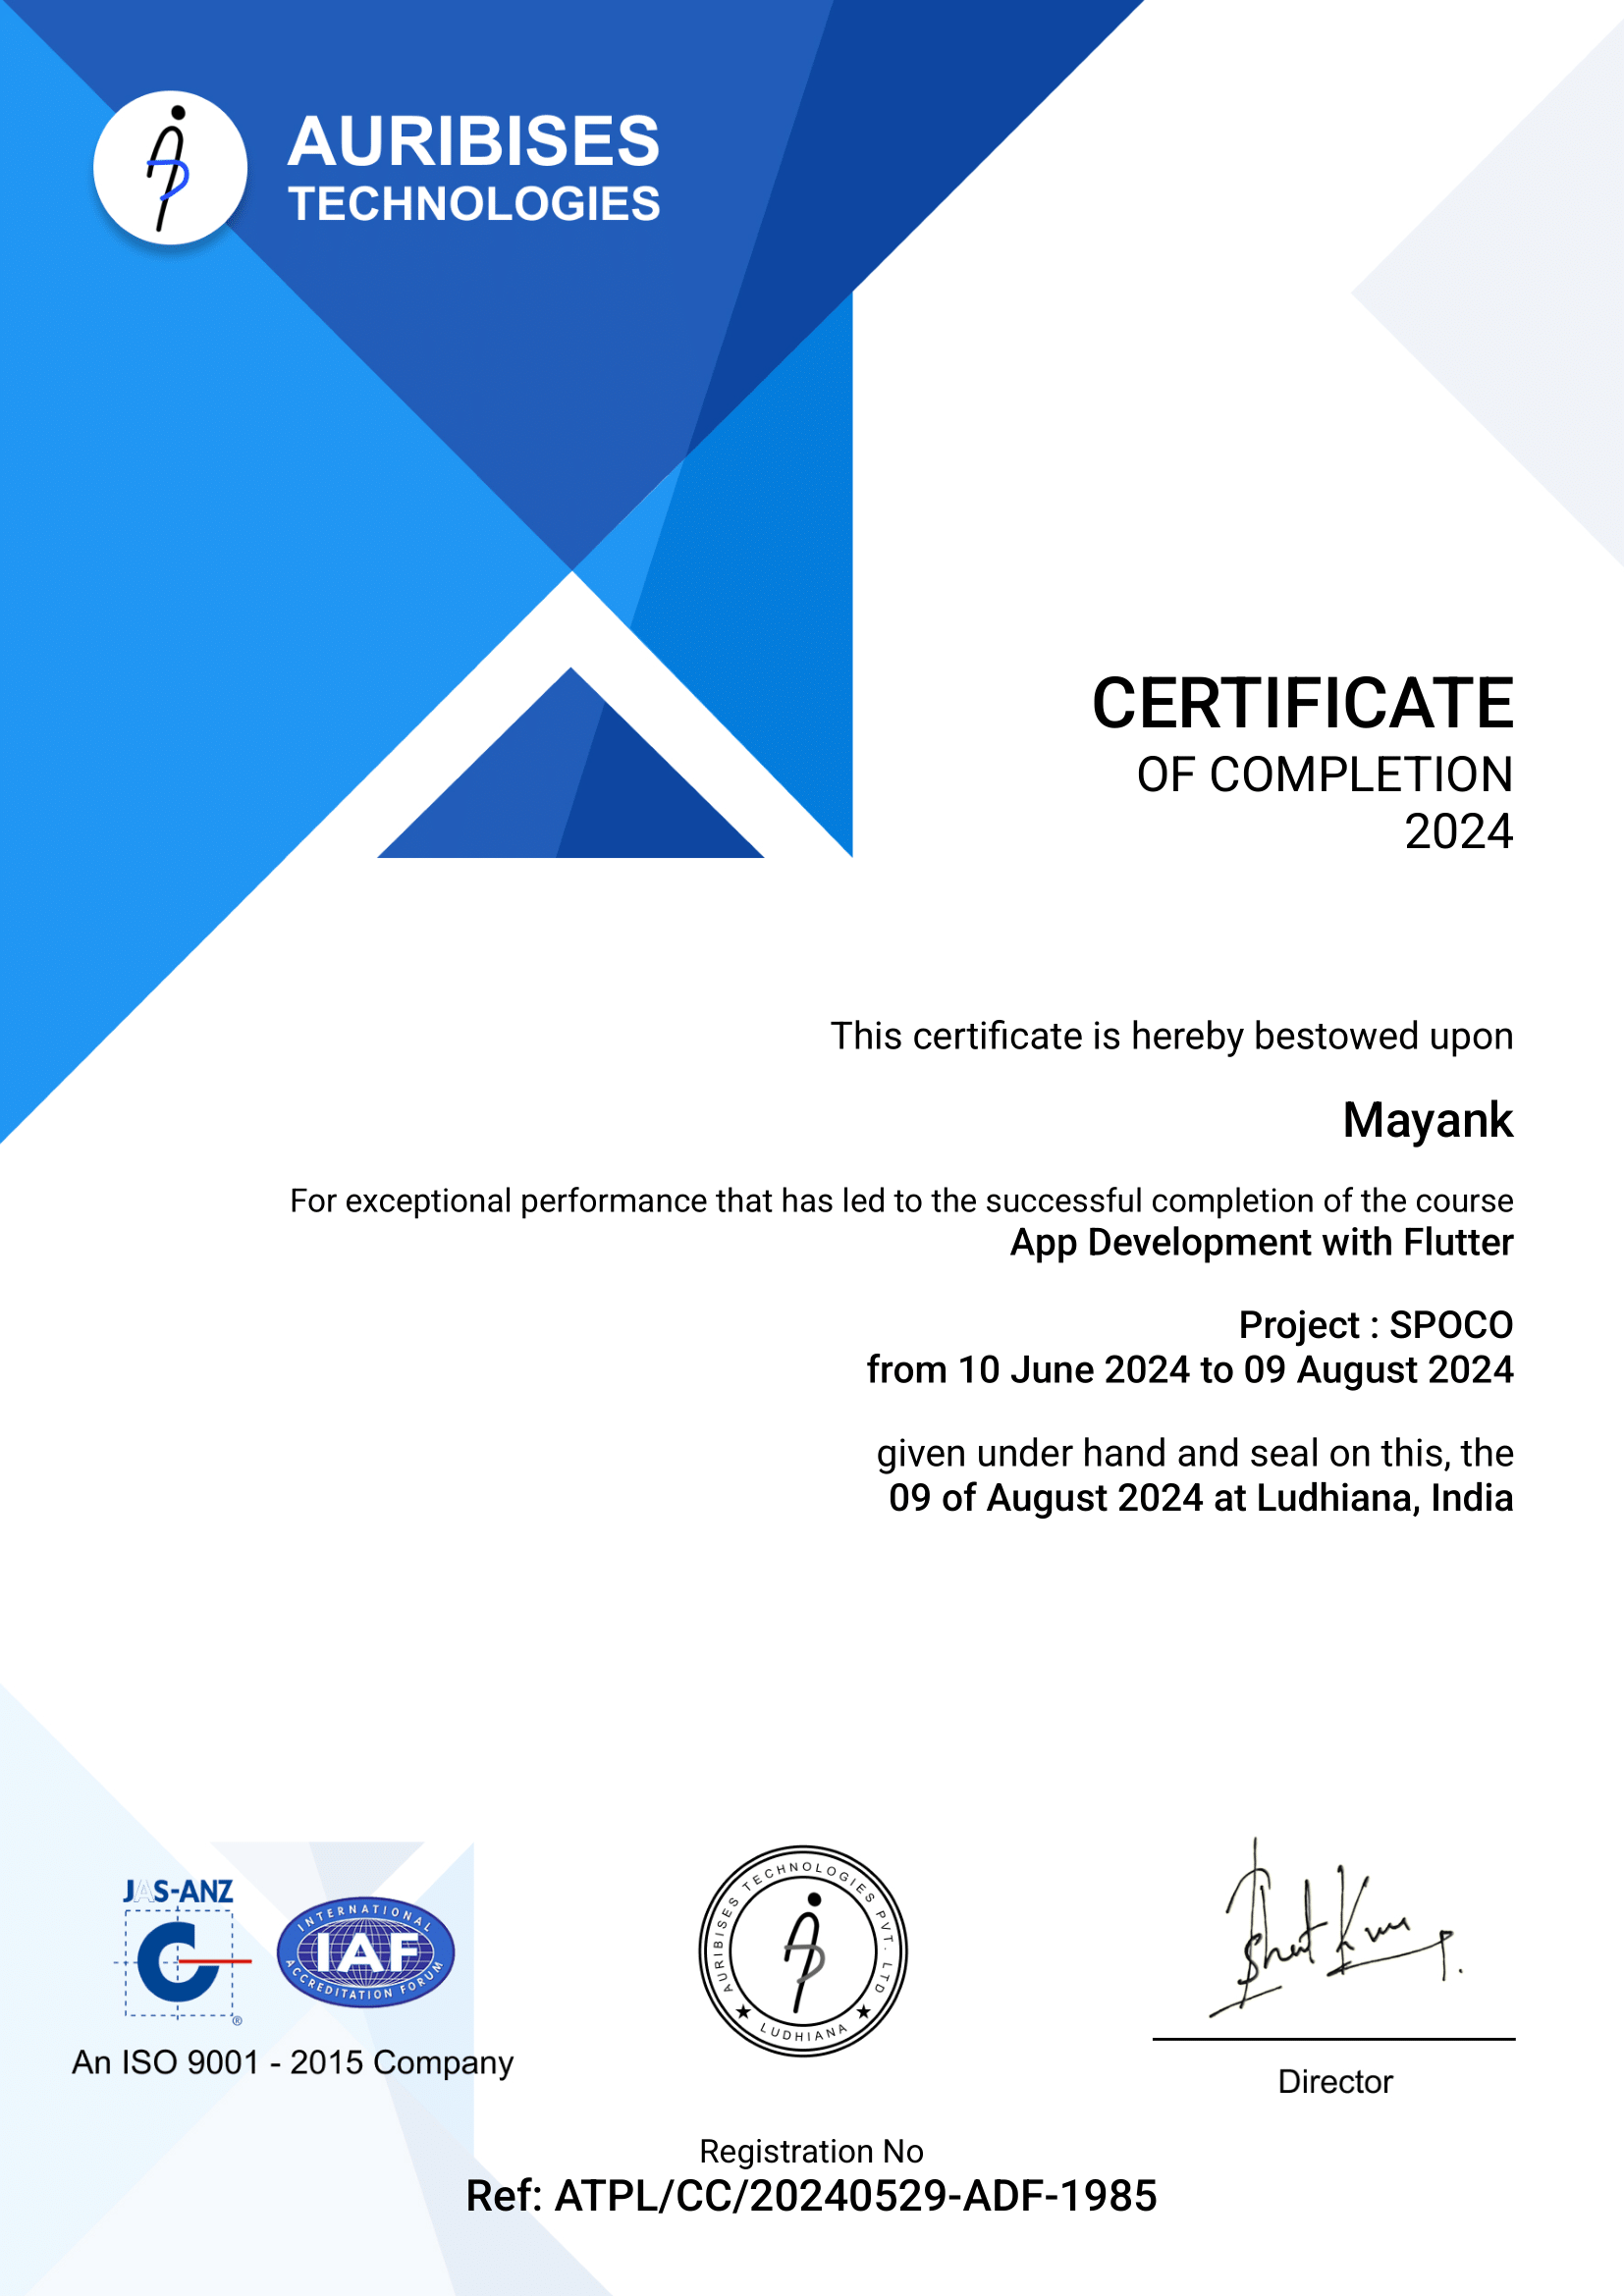
\includegraphics[width=1\textwidth]{assets/certificate.png}
\end{center}

\newpage

\chapter*{}
\addcontentsline{toc}{chapter}{Candidate's Declaration} 
% Declaration Page
\begin{center}
    \textbf{GURU NANAK DEV ENGINEERING COLLEGE, LUDHIANA}\\ \vspace{1cm}
    \textbf{CANDIDATE'S DECLARATION}
\end{center}
\vspace{1cm}
I, \textbf{Mayank}, hereby declare that I have undertaken four week training "\textit Auribises Technologies Pvt Ltd" during a period from {10.06.2024} to {09.08.2024} in partial fulfillment of requirements for the award of degree of B.Tech (Information Technology) at GURU NANAK DEV ENGINEERING COLLEGE, LUDHIANA. The work which is being presented in the training report submitted to Department of Information Technology at GURU NANAK DEV ENGINEERING COLLEGE, LUDHIANA is an authentic record of training work.

\vspace{3cm}
\begin{flushleft}
    Signature of the Student\\
\end{flushleft}

\vspace{2cm}
The four week industrial training Viva-Voce Examination of \underline{\hspace{5cm}} has been held on \underline{\hspace{3cm}} and accepted.

\vspace{3cm}
\begin{tabbing}
    Signature of Internal Examiner \hspace{4cm} \= Signature of External Examiner
\end{tabbing}

\newpage

\chapter*{}
\addcontentsline{toc}{chapter}{Abstract}  
% Abstract Page
\begin{center}
    \textbf{ABSTRACT}
\end{center}
This report presents an overview of my training experience in Mobile App Development using Flutter, conducted by Auribises Technologies Pvt Ltd under the mentorship of \textbf{Ishant Kumar}. The training program focused on essential concepts such as Dart programming, Flutter frameworks, Firebase integration, UI/UX design principles, and state management techniques. As a key project, I contributed to the development of the \textbf{SPOCO} app, a live platform designed for users to discover and book sports grounds efficiently.
My responsibilities included defining Firebase collection paths, building the authentication module, implementing turf management functionalities, and developing the event booking system. This hands-on experience allowed me to apply theoretical knowledge in a practical context, fostering teamwork and enhancing my problem-solving skills.
The report is structured into four chapters: an introduction to the training course and its objectives, a detailed overview of the training work undertaken, a discussion of the \textbf{SPOCO} app and its functionalities, and conclusions with suggestions for future enhancements. The training not only enriched my technical expertise but also prepared me for future challenges in mobile application development, equipping me with the skills necessary to create user-centric, cross-platform applications.
% This report outlines the work undertaken during four weeks of training at AV Communications, with a focus on mobile application development using Flutter. The training provided practical experience in building cross-platform mobile apps, emphasizing key concepts like state management, offline storage, and UI/UX design. The primary project, \textbf{Split It}, was developed as a tool to help users track and manage shared expenses, incorporating technologies like the Isar database for offline data handling and Riverpod for state management.

% Throughout the training, I gained valuable skills in using Flutter’s widget-based architecture, designing intuitive user interfaces, and integrating efficient data storage solutions. The hands-on nature of the project helped reinforce the theoretical concepts of mobile development, allowing me to understand the importance of responsive design, clean architecture, and app optimization. Tools like Git for version control and Flutter DevTools for testing and debugging were also integral parts of the development process.

% The report concludes with insights into future improvements for the \textbf{Split It} app, such as adding cloud sync functionality, payment integration, and enhanced collaboration features. This training has laid a strong foundation for further growth in mobile development and has equipped me with the tools necessary to tackle more advanced projects.

\newpage


\chapter*{}
\addcontentsline{toc}{chapter}{Acknowledgement} 
% Acknowledgment Page
\begin{center}
    \textbf{ACKNOWLEDGMENT}
\end{center}
I would like to express my sincere gratitude to \textbf{Auribises Technologies Pvt. Ltd.} for providing me with the opportunity to carry out my training and gain valuable insights into mobile application development. This experience has been instrumental in enhancing my practical skills, and I am especially thankful for the guidance and support provided by my training supervisor, whose expertise and encouragement were crucial throughout the project. I would also like to acknowledge the staff at Auribises Technologies Pvt Ltd for creating a collaborative learning environment and for their willingness to assist me whenever needed.

Furthermore, I extend my heartfelt thanks to the faculty members of \textbf{Guru Nanak Dev Engineering College}, whose continuous encouragement and support helped me undertake this training with confidence. Their mentorship has been pivotal in my academic growth, and I am grateful for the foundation they provided, which allowed me to fully benefit from this practical experience. This training has been an invaluable step in my journey, and I deeply appreciate all the individuals who contributed to its success.

\newpage

% List of Figures and Tables (Optional)
\chapter*{}
\addcontentsline{toc}{chapter}{List of Figures} 
\listoffigures
\chapter*{}
\addcontentsline{toc}{chapter}{List of Tables} 
\listoftables
\newpage

\setcounter{tocdepth}{1}
\setlength{\cftbeforechapskip}{0pt} 
\setlength{\cftbeforesecskip}{0pt} 
\setlength{\cftbeforetoctitleskip}{-1em} 
\tableofcontents

\pagenumbering{arabic}

% Chapter 1: Introduction
\chapter{Introduction}
\setstretch{1.5}

\section{Background}
The training undertaken at \textbf{Auribises Technologies Pvt Ltd} focused on mobile application development using Flutter. Flutter is an open-source UI software development toolkit created by Google, which is used to develop natively compiled applications for mobile, web, and desktop from a single codebase. The training provided a comprehensive introduction to Flutter, covering both theoretical and practical aspects of mobile application development.

Auribises Technologies Pvt Ltd, a company specializing in communication and electronic solutions, provided a structured learning experience aimed at familiarizing trainees with industry-level practices for developing modern mobile applications. The company offered exposure to the complete software development lifecycle, including requirements gathering, design, implementation, testing, and deployment of mobile applications.

\subsection{Theoretical Explanation}
Flutter is based on the Dart programming language, which was also developed by Google. Dart is optimized for building user interfaces, making it an ideal choice for Flutter. Flutter’s architecture comprises several layers, including the framework layer, engine layer, and embedded layer. The framework layer contains a rich set of pre-designed widgets, while the engine layer, built in C++, provides low-level rendering using Skia. The embedded layer integrates Flutter applications into the platform-specific environment.

The training involved learning about Flutter's core concepts, such as widgets, state management, navigation, and animations. Widgets are the building blocks of Flutter applications, and understanding their usage and customization is crucial for creating dynamic and responsive UIs. State management, which refers to managing the state of the application’s UI, was also a key focus. Various approaches to state management, such as using Provider or Riverpod, were introduced during the training.

Another important topic covered was navigation, which involves managing the movement between different screens of an application. Flutter provides a flexible navigation system that can be customized to suit various app requirements. Animations, which enhance user experience by adding visual feedback and transitions, were also explored in detail. Different types of animations, including implicit and explicit animations, were implemented to understand their impact on user interaction.

\subsubsection{Overview of Mobile App Development Approaches}

When it comes to mobile app development, developers can choose from multiple approaches based on the requirements of their project, the desired user experience, and available resources. The three most common approaches are:

\paragraph{Native Development:}
Native development involves writing platform-specific applications using the officially supported languages and tools for each operating system. For Android, this means using Java or Kotlin, while for iOS, it involves Swift or Objective-C. Native development provides full access to the device’s hardware and platform-specific APIs, resulting in the best possible performance and user experience. However, this approach requires maintaining separate codebases for Android and iOS, leading to increased development time and maintenance complexity.

\paragraph{Flutter:}
Flutter is a cross-platform development framework created by Google. It allows developers to build natively compiled applications for multiple platforms (Android, iOS, web, and desktop) using a single codebase written in Dart. Flutter is known for its rich set of pre-designed widgets and hot reload feature, which accelerates the development process. Flutter applications offer near-native performance and provide a consistent user interface across platforms, although advanced platform-specific features may require custom native code.

\paragraph{React Native:}
React Native, developed by Facebook, is another cross-platform framework that allows developers to write mobile applications for both Android and iOS using JavaScript and React. Like Flutter, it enables the reuse of a single codebase for multiple platforms. React Native relies on a JavaScript bridge to communicate with native components, which can sometimes lead to performance bottlenecks, though it is still suitable for many types of applications. React Native’s large ecosystem and its foundation in JavaScript make it popular among web developers looking to transition to mobile development.

\paragraph{Summary:}
Each approach has its strengths and trade-offs:
\begin{itemize}
    \item \textbf{Native development} offers the best performance and platform-specific capabilities but requires maintaining separate codebases.
    \item \textbf{Flutter} offers a single codebase for multiple platforms with near-native performance and a unified UI, making it an efficient choice for many projects.
    \item \textbf{React Native} also allows cross-platform development with a single codebase, leveraging JavaScript and React, but may have slight performance limitations compared to native and Flutter applications.
\end{itemize}

Choosing the right approach depends on factors such as project complexity, performance needs, time constraints, and available resources.


\subsubsection{Comparison Between Native, Flutter, and React Native App Development}

When developing mobile applications, developers can choose between different frameworks and technologies. Each option comes with its own strengths and trade-offs. The three main approaches are:

\begin{itemize}
    \item \textbf{Native Development:} Using platform-specific languages like Java or Kotlin for Android, and Swift or Objective-C for iOS.
    \item \textbf{Flutter:} A cross-platform framework by Google that uses Dart to build apps for multiple platforms from a single codebase.
    \item \textbf{React Native:} A cross-platform framework by Facebook that uses JavaScript and React to build apps for both Android and iOS.
\end{itemize}


The table below compares these three approaches based on various key factors:

\begin{table}
\centering
\begin{tabular}{|p{3cm}|p{4cm}|p{4cm}|p{4cm}|}
\hline
\textbf{Aspect} & \textbf{Native Development (Java/Swift/Kotlin)} & \textbf{Flutter} & \textbf{React Native} \\ \hline
\textbf{Performance} & Best performance due to direct native code compilation and platform APIs. & Near-native performance with Dart-to-native code and Skia engine. & Slightly lower performance due to JavaScript bridge, but still suitable for most apps. \\ \hline
\textbf{Codebase} & Separate codebases for Android and iOS, increasing maintenance. & Single codebase for Android, iOS, and more, reducing maintenance. & Single codebase for Android and iOS, reducing development time. \\ \hline
\textbf{UI Components} & Full access to native UI components with platform-specific behavior. & Custom UI layer with Flutter widgets, offering consistent UI across platforms. & Uses native components but may need custom modules for certain features. \\ \hline
\textbf{Learning Curve} & Steeper as it requires learning both Java/Kotlin and Swift. & Easier with a single language (Dart) and widget system. & Easier for those familiar with JavaScript and React but may require native module knowledge. \\ \hline
\textbf{Development Speed} & Slower due to managing separate platforms and testing processes. & Faster with a single codebase and hot reload for quick testing. & Faster with single codebase and hot reloading, but bridging can slow development. \\ \hline
\textbf{Ecosystem} & Extensive, with mature libraries and tools for Android and iOS. & Growing, with an expanding library ecosystem and strong support from Google. & Large due to JavaScript and React, but may require third-party libraries for native functionality. \\ \hline
\textbf{UI Consistency} & Perfect platform-specific consistency. & Consistent UI across platforms, but may need customization for platform guidelines. & Mostly consistent, but can vary depending on native components. \\ \hline
\textbf{Native Features} & Full access to native APIs and features. & Access through plugins; custom native code may be required for some features. & Access via native modules; complex features may require custom bridging. \\ \hline
\textbf{Community} & Strong, with well-established support and documentation. & Growing fast with active support and development. & Large community due to JavaScript and React, with good support and resources. \\ \hline
\textbf{Platforms} & Platform-specific (Android and iOS) with separate apps. & Cross-platform (Android, iOS, web, desktop) from a single codebase. & Cross-platform (Android and iOS) from a single codebase; limited web support. \\ \hline
\end{tabular}
\caption{Comparison Between Native, Flutter, and React Native App Development}
\end{table}



\subsection{Software and Hardware Tools Learned}
The training primarily focused on software tools, with some hardware tools integrated to facilitate mobile application development. The key software tools I gained experience with during the development of the spoco included

\begin{itemize}
    \item \textbf{Flutter SDK:} The Flutter Software Development Kit (SDK) was the main tool used for building mobile applications. It provided the necessary libraries and tools to create and test Flutter applications.
    \item \textbf{Visual Studio Code:} As the Integrated Development Environment (IDE), I used VS Code to write, debug, and run Flutter code. It provided powerful extensions for Flutter and Dart development, offering features for code editing, debugging, and UI design.
    \item \textbf{ Firebase Services:}  Firebase Firestore was integrated for real-time data storage and synchronization, while Firebase Authentication was utilized to manage secure user logins. Firebase Storage was employed to store and retrieve user-uploaded files, such as images.
    \item Various Flutter Libraries such as 
    \begin{itemize}
        \item \textbf{Provider:} A popular package for state management used to manage application states across different widgets, providing flexibility and making the app easier to maintain.
        \item \textbf{ ENSwiper:} A library that simplified the process of implementing card-based swiping functionality for browsing turf options.
        \item \textbf{URL Launcher:} A package used to open URLs (like Google Maps) from within the app, enabling users to access location details for different sports facilities directly.

    \end{itemize}
\end{itemize}

\subsection{Objectives of the Training}
The objectives of this training were as follows:
\begin{itemize}
    \item To understand the fundamentals of mobile application development using Flutter.
    \item To gain hands-on experience in using Flutter to create cross-platform mobile applications.
    \item To learn about the complete software development lifecycle, from design to deployment, for mobile applications.
    \item To understand the use of state management, navigation, and animations in building modern mobile apps.
    \item To become familiar with integrating backend services using Firebase.
\end{itemize}

The training aimed to equip the trainee with the knowledge and skills necessary to create industry-standard mobile applications using Flutter. By the end of the training, the trainee was expected to have a strong understanding of the development tools and practices required for mobile app development and to be capable of contributing effectively to real-world mobile projects.

\section{The Dart Programming Language}
Dart is the programming language used for developing Flutter applications. Created by Google, Dart is optimized for client-side development, specifically for building fast, responsive user interfaces. It is a versatile language that supports object-oriented programming, functional programming, and asynchronous programming, making it highly suitable for modern application development.

\subsection{Features of Dart}
Dart offers a number of features that make it ideal for mobile application development:
\begin{itemize}
    \item \textbf{Object-Oriented Programming:} Dart is a class-based, object-oriented language. It uses classes and objects to structure code, making it easy to model real-world entities in applications. In Flutter, widgets are typically structured as classes, demonstrating the importance of Dart’s OOP capabilities.
    
    \item \textbf{Asynchronous Programming:} Dart supports asynchronous programming through the use of \texttt{async} and \texttt{await} keywords. This is crucial for handling time-consuming tasks like fetching data from the internet or reading files, allowing the application to remain responsive while waiting for operations to complete.
    
    \item \textbf{Null Safety:} Dart enforces null safety by ensuring that variables can’t be null unless explicitly declared as nullable. This helps prevent a common class of bugs caused by null values, making code more robust and easier to maintain.
    
    \item \textbf{Ahead-of-Time (AOT) and Just-in-Time (JIT) Compilation:} Dart can be compiled both ahead-of-time (AOT) and just-in-time (JIT). AOT compilation is used for production builds, resulting in fast, natively compiled applications. JIT compilation is utilized during development to provide faster iterations by enabling hot reload, allowing developers to see changes in real time without restarting the application.
    
    \item \textbf{Garbage Collection:} Dart includes an automatic memory management system, or garbage collector, which helps manage memory allocation and deallocation. This ensures that unused memory is released, reducing the likelihood of memory leaks in applications.
\end{itemize}

\subsection{Dart’s Role in Flutter Development}
Dart plays a central role in Flutter development by serving as both the programming language for writing Flutter applications and the backbone of the Flutter framework. Dart’s syntax is easy to read and learn, which makes it accessible to both beginner and experienced developers. Flutter uses Dart’s declarative style to build user interfaces, meaning developers describe how the UI should look in terms of widgets, and Dart handles the process of rendering and updating these widgets efficiently.

Additionally, Dart’s rich set of core libraries includes support for working with collections, dates, JSON parsing, and more, which simplifies many common tasks in mobile app development. Dart’s powerful async features also align well with Flutter’s reactive programming model, where user interface updates are triggered by changes in the app’s state.

\subsection{Dart Syntax and Example Code}

Dart’s syntax is similar to other C-style languages, making it easy for developers to pick up. In this section, we will explore some key syntax elements and example code to demonstrate the basics of Dart programming.

\subsubsection{Variables and Data Types}
In Dart, variables can be defined using the \texttt{var}, \texttt{final}, or \texttt{const} keywords. The data type can either be inferred or explicitly defined.

\begin{lstlisting}[language=Dart, caption={Dart Variables and Data Types}]
var name = 'Flutter';
String framework = 'Flutter';

final int version = 3;
const String author = 'Google';
\end{lstlisting}

The key difference between \texttt{final} and \texttt{const} is that \texttt{const} variables are compile-time constants, while \texttt{final} variables can be assigned only once but may be determined at runtime.

\subsubsection{Functions}
Functions in Dart are defined using the \texttt{void} keyword for functions that don’t return a value, or by specifying the return type for functions that do return a value.

\begin{lstlisting}[language=Dart, caption={Functions in Dart}]
// Function without a return value
void printGreeting(String name) {
    print('Hello, $name!');
}

// Function with a return value
int add(int a, int b) {
    return a + b;
}

// Arrow function syntax for short functions
int multiply(int a, int b) => a * b;
\end{lstlisting}

\subsubsection{Control Flow Statements}
Dart supports common control flow statements like \texttt{if-else}, \texttt{for}, \texttt{while}, and \texttt{switch}.

\begin{lstlisting}[language=Dart, caption={Control Flow Statements in Dart}]
int number = 10;
if (number > 5) {
    print('Greater than 5');
} else {
    print('Less than or equal to 5');
}

for (int i = 0; i < 5; i++) {
    print(i);
}

String grade = 'A';
switch (grade) {
  case 'A':
    print('Excellent');
    break;
  case 'B':
    print('Good');
    break;
  default:
    print('Try harder');
}
\end{lstlisting}

\subsubsection{Classes and Objects}
Dart is an object-oriented language, and classes are the blueprint for creating objects. A class in Dart can contain fields, constructors, methods, and even static members.

\begin{lstlisting}[language=Dart, caption={Classes and Objects in Dart}]
// Class definition
class Car {
  String brand;
  int year;

  // Constructor
  Car(this.brand, this.year);

  // Method
  void displayInfo() {
    print('Brand: $brand, Year: $year');
  }
}

// Creating an object
void main() {
  var car = Car('Toyota', 2021);
  car.displayInfo();
}
\end{lstlisting}

In the example above, we define a \texttt{Car} class with a constructor and a method. We create an object of the \texttt{Car} class and call the method to display the car's information.

\subsubsection{Asynchronous Programming}
Asynchronous operations in Dart are handled using the \texttt{Future} class and \texttt{async} and \texttt{await} keywords. This allows you to perform tasks that take time (like API calls) without blocking the execution of other code.

\begin{lstlisting}[language=Dart, caption={Asynchronous Programming in Dart}]
Future<String> fetchData() async {
    await Future.delayed(Duration(seconds: 2));
    return 'Data fetched';
}

void main() async {
    print('Fetching data...');
    String result = await fetchData();
    print(result);
}
\end{lstlisting}


The example shows how the \texttt{fetchData()} function simulates an asynchronous operation, and the \texttt{await} keyword is used to wait for the result before proceeding.

\subsubsection{Collections}
Dart offers powerful built-in collection types, such as \texttt{List}, \texttt{Set}, and \texttt{Map}, for managing groups of objects.

\begin{lstlisting}[language=Dart, caption={Collections in Dart}]
// List
List<String> fruits = ['Apple', 'Banana', 'Mango'];
fruits.add('Orange');
print(fruits); // ['Apple', 'Banana', 'Mango', 'Orange']

// Set (no duplicates allowed)
Set<int> numbers = {1, 2, 3, 3};
print(numbers); // {1, 2, 3}

// Map
Map<String, int> scores = {'Alice': 90, 'Bob': 85};
print(scores['Alice']); // 90
\end{lstlisting}

Lists in Dart are ordered, Sets are unordered and disallow duplicates, and Maps store key-value pairs.

\subsubsection{Null Safety}
Dart’s null safety feature ensures that variables cannot contain null values unless explicitly declared as nullable using the \texttt{?} symbol.

\begin{lstlisting}[language=Dart, caption={Null Safety in Dart}]
// Non-nullable variable
int age = 25;

// Nullable variable
int? nullableAge;

// Safe access to nullable variables
nullableAge?.toString();  // Returns null if nullableAge is null
\end{lstlisting}

This feature significantly reduces runtime errors by preventing null dereference errors.

\subsubsection{Exception Handling}
Dart handles errors and exceptions using \texttt{try}, \texttt{catch}, and \texttt{finally} blocks.

\begin{lstlisting}[language=Dart, caption={Exception Handling in Dart}]
void main() {
    try {
        int result = 10 ~/ 0; // Integer division by zero
    } catch (e) {
        print('Error: $e');
    } finally {
        print('Cleanup code');
    }
}
\end{lstlisting}

In this example, we handle an integer division by zero, catch the exception, and ensure that the \texttt{finally} block runs regardless of whether an exception occurs.


\subsection{Use of Dart During the Training}
During the training, Dart was used extensively for writing the business logic and user interface of the mobile applications being developed. Key Dart features such as asynchronous programming were explored through handling API calls and performing real-time updates. The introduction of null safety in Dart 2.12 was also a significant focus, as it helped prevent potential runtime errors and made the code more reliable.

The training emphasized writing clean, maintainable code using Dart’s object-oriented features, and best practices for organizing Dart files and classes in Flutter projects. Dart's integration with Flutter also facilitated rapid development, allowing us to take full advantage of hot reload for efficient debugging and testing.

Overall, Dart proved to be a highly effective language for developing mobile applications, providing the necessary tools and features to build high-quality, performance-driven apps.

\section{The Flutter SDK}
The Flutter Software Development Kit (SDK) is an open-source framework developed by Google for building natively compiled applications for mobile, web, and desktop from a single codebase. The SDK provides all the necessary tools, libraries, and APIs to create highly performant and visually attractive applications with a consistent user experience across platforms.

Flutter uses the Dart programming language and leverages a rich set of pre-designed widgets, a reactive UI framework, and a rendering engine to enable developers to build and test applications efficiently.

\subsubsection{Flutter Basics: A Simple "Hello World" App}

Flutter is a cross-platform UI toolkit that enables developers to build natively compiled applications for mobile, web, and desktop using a single codebase. At the core of Flutter's design is its use of widgets, which are the fundamental building blocks of a Flutter application. Every element in a Flutter app, from buttons and text to layouts and containers, is a widget.

To get started, here’s a simple "Hello World" application in Flutter. This app demonstrates how to create a basic Flutter app with a text widget displayed in the center of the screen.

\paragraph{Example: Hello World in Flutter}

\begin{lstlisting}[language=Dart, caption={Flutter Hello World App}]
import 'package:flutter/material.dart';

void main() {
  runApp(const MyApp());
}

class MyApp extends StatelessWidget {
  const MyApp({Key? key}) : super(key: key);

  @override
  Widget build(BuildContext context) {
    return MaterialApp(
      home: Scaffold(
        appBar: AppBar(
          title: const Text('Hello World App'),
        ),
        body: const Center(
          child: Text('Hello, World!'),
        ),
      ),
    );
  }
}
\end{lstlisting}

\paragraph{Explanation:}
This simple Flutter app consists of the following key components:
\begin{itemize}
    \item \textbf{main() function:} The entry point of the Flutter app, where the \texttt{runApp()} function initializes the app by inflating the widget tree.
    \item \textbf{MyApp class:} A \texttt{StatelessWidget} that returns a \texttt{MaterialApp}, which is the root widget of the app. The \texttt{MaterialApp} provides material design elements.
    \item \textbf{Scaffold:} A layout structure used for creating material design apps. It contains an app bar at the top and a body where the content (in this case, a centered text widget) is placed.
    \item \textbf{Text widget:} The \texttt{Text} widget is used to display the "Hello, World!" string in the center of the screen.
\end{itemize}

\paragraph{Basic Concepts:}
\begin{itemize}
    \item \textbf{Widgets:} In Flutter, everything is a widget. Widgets describe how the UI should look, and Flutter uses a declarative approach to build the UI. Widgets can be either \texttt{Stateless} (which don’t maintain state) or \texttt{Stateful} (which can change state over time).
    \item \textbf{Hot Reload:} One of Flutter's most powerful features, hot reload allows developers to see changes in the app in real-time, making the development process faster and more efficient.
\end{itemize}

This simple "Hello World" app demonstrates the basic structure of a Flutter application and introduces the concept of widgets, which are crucial in Flutter development.


\subsection{Key Components of the Flutter SDK}
The Flutter SDK consists of several key components that make it a powerful framework for cross-platform development:

\subsubsection{Widgets}
Widgets are the fundamental building blocks of Flutter applications. Everything in Flutter is a widget, including layouts, buttons, text, and even the entire app itself. Widgets can be composed to create complex UIs, and Flutter provides a wide range of pre-built widgets to simplify common tasks.

\begin{lstlisting}[language=Dart, caption={Simple Flutter Widget}]
Widget build(BuildContext context) {
  return Text('Hello, Flutter!');
}
\end{lstlisting}

In this example, the \texttt{Text} widget is used to display a simple string. The \texttt{build} method is a core part of the widget lifecycle, responsible for constructing the widget tree that defines the UI.

\subsubsection{Hot Reload}
One of Flutter's standout features is \textbf{Hot Reload}, which allows developers to see changes in the code immediately, without needing to restart the entire application. Hot reload is especially useful for tweaking UIs, fixing bugs, and experimenting with new ideas quickly.

\subsubsection{Declarative UI Programming}
Flutter employs a declarative programming style, where developers describe the UI using widgets, and the framework handles updating the UI when the app's state changes. This contrasts with the imperative style used in other frameworks, which requires manual UI updates.

\begin{lstlisting}[language=Dart, caption={Declarative UI Example}]
@override
Widget build(BuildContext context) {
  return Column(
    children: [
      Text('Welcome'),
      ElevatedButton(
        onPressed: () => print('Button Pressed'),
        child: Text('Press Me'),
      ),
    ],
  );
}
\end{lstlisting}

In this example, the UI consists of a column with a text label and a button. The button triggers a print statement when pressed, and the declarative style allows Flutter to automatically manage UI changes when the state is updated.

\subsubsection{Flutter Engine}
The Flutter engine, written in C++, is responsible for rendering the UI and executing the Dart code. It uses Skia, a 2D graphics library, to render widgets and handle animations. This engine is platform-agnostic, which is why Flutter applications can run on iOS, Android, web, and desktop with minimal platform-specific code.

\subsection{State Management in Flutter SDK}
Managing the state of an application efficiently is a critical aspect of Flutter development. Flutter offers several state management solutions, such as:
\begin{itemize}
    \item \textbf{setState:} A simple method for updating the state within a widget. It works well for small, self-contained components but becomes challenging to scale in large applications.
    \item \textbf{Provider:} A more scalable solution for managing state, it allows sharing data across different parts of the application, following a reactive approach.
    \item \textbf{Riverpod:} An enhanced state management library that improves upon Provider’s features, providing a more flexible and testable way to manage dependencies and state.
\end{itemize}

\begin{lstlisting}[language=Dart, caption={Simple setState Example}]
class Counter extends StatefulWidget {
  @override
  _CounterState createState() => _CounterState();
}

class _CounterState extends State<Counter> {
  int count = 0;

  @override
  Widget build(BuildContext context) {
    return Column(
      children: [
        Text('Count: $count'),
        ElevatedButton(
          onPressed: () => setState(() {
            count++;
          }),
          child: Text('Increment'),
        ),
      ],
    );
  }
}
\end{lstlisting}

In this example, the \texttt{setState} method is used to update the UI when the button is pressed, causing the counter to increment and re-render the text.

\subsection{Stateless Widgets}
In Flutter, widgets are divided into two main categories: \textbf{Stateless} and \textbf{Stateful} widgets. A \textbf{StatelessWidget} is a widget that does not require any mutable state. This means that once a StatelessWidget is built, it will not change over time unless an external factor (such as a parent widget) forces it to rebuild. Stateless widgets are ideal for static content or UI elements that do not need to react to user interactions.

\textbf{Example:}

\begin{lstlisting}[language=Dart, caption={Example of a Stateless Widget}]
class MyStatelessWidget extends StatelessWidget {
  @override
  Widget build(BuildContext context) {
    return Center(
      child: Text('I am a stateless widget'),
    );
  }
}
\end{lstlisting}

In this example, the widget displays a simple text string. Since this widget doesn’t need to respond to changes or interactions, it remains static, which makes it a good use case for a StatelessWidget.

\textbf{Key Characteristics of Stateless Widgets:}
\begin{itemize}
    \item The widget cannot change its state after being built.
    \item It’s ideal for displaying static content like text, icons, and images.
    \item The \texttt{build} method is called only once unless the parent widget requests a rebuild.
\end{itemize}

\subsection{Stateful Widgets}
Unlike StatelessWidgets, \textbf{StatefulWidgets} can change over time in response to user interactions or other factors. A StatefulWidget has mutable state, meaning that it can update its appearance and behavior dynamically. This is achieved by using a separate class to manage the widget's state, which is represented by the \texttt{State} object. 

When a StatefulWidget's state changes, Flutter calls the \texttt{setState} method to trigger a rebuild, allowing the UI to reflect the updated state.

\textbf{Example:}

\begin{lstlisting}[language=Dart, caption={Example of a Stateful Widget}]
class MyStatefulWidget extends StatefulWidget {
  @override
  _MyStatefulWidgetState createState() => _MyStatefulWidgetState();
}

class _MyStatefulWidgetState extends State<MyStatefulWidget> {
  int counter = 0;

  void incrementCounter() {
    setState(() {
      counter++;
    });
  }

  @override
  Widget build(BuildContext context) {
    return Column(
      mainAxisAlignment: MainAxisAlignment.center,
      children: [
        Text('Counter: $counter'),
        ElevatedButton(
          onPressed: incrementCounter,
          child: Text('Increment'),
        ),
      ],
    );
  }
}
\end{lstlisting}

In this example, the widget displays a counter that increments each time the button is pressed. The \texttt{setState} method is used to update the counter, which triggers a UI rebuild, showing the new counter value.

\textbf{Key Characteristics of Stateful Widgets:}
\begin{itemize}
    \item The widget has mutable state and can change dynamically.
    \item Ideal for components that need to respond to user input, animations, or other interactions.
    \item The \texttt{setState} method is used to update the widget's state and trigger a rebuild.
    \item The widget is rebuilt whenever its state changes, allowing for dynamic content updates.
\end{itemize}

\subsection{Differences Between Stateless and Stateful Widgets}
Stateless and Stateful Widgets are the primary building blocks of any flutter app and being able to understand the differences and use case of each is integral to be able to design and develop apps effectively with flutter.

The main differences between \textbf{Stateless} and \textbf{Stateful} widgets can be summarized in the following table:

\begin{table}[H]
\centering
\begin{tabular}{|p{4cm}|p{5cm}|p{5cm}|}
\hline
\textbf{Aspect} & \textbf{StatelessWidget} & \textbf{StatefulWidget} \\ \hline
\textbf{State} & No mutable state. Once built, it remains static. & Has mutable state that can change over time during the widget's lifecycle. \\ \hline
\textbf{Use Cases} & Best for static content that doesn’t change, such as text, images, icons, etc. & Ideal for dynamic content or interactive components like forms, buttons, sliders, and animations. \\ \hline
\textbf{Rebuilds} & Rebuilt only when the parent widget requests a rebuild. & Can rebuild itself when its internal state changes, using \texttt{setState()}. \\ \hline
\textbf{Performance} & Slightly more performant since the widget doesn’t need to manage state. & Slightly less performant due to state management overhead. \\ \hline
\textbf{Lifecycle Methods} & Has only a \texttt{build()} method. & Includes multiple lifecycle methods such as \texttt{initState()}, \texttt{setState()}, and \texttt{dispose()}. \\ \hline
\end{tabular}
\caption{Comparison between Stateless and Stateful Widgets}
\end{table}

\subsection{Flutter’s Ecosystem}
The Flutter SDK also benefits from a vibrant ecosystem of tools and libraries:
\begin{itemize}
    \item \textbf{Flutter DevTools:} A suite of performance and debugging tools specifically designed for Flutter applications.
    \item \textbf{DartPad:} An online code editor that allows developers to experiment with Dart and Flutter code directly in the browser without needing to install the SDK.
    \item \textbf{Pub.dev:} A central repository for discovering and integrating third-party Flutter and Dart libraries into your projects.
\end{itemize}

\subsection{Advantages of Using Flutter SDK}
There are several advantages to using the Flutter SDK for mobile application development:
\begin{itemize}
    \item \textbf{Cross-Platform Development:} Flutter allows developers to write a single codebase that compiles natively for multiple platforms, saving both time and resources.
    \item \textbf{Fast Development:} Features like hot reload, a rich set of pre-built widgets, and a declarative UI framework enable developers to build applications quickly and efficiently.
    \item \textbf{Native Performance:} Flutter compiles directly to native code, which ensures high performance across platforms.
    \item \textbf{Customizable UI:} The flexibility of Flutter’s widget system allows developers to create highly customizable UIs that closely match platform-specific design guidelines.
\end{itemize}

\subsection{Conclusion}
The Flutter SDK is a robust tool for developing cross-platform applications with a modern and efficient approach. Its combination of a reactive UI framework, an extensive ecosystem, and support for hot reload makes it a powerful choice for developers looking to create high-quality mobile applications quickly. The training covered both the theoretical foundations and hands-on experience with Flutter, preparing developers to build performant, maintainable applications with ease.


\chapter{Training Work Undertaken}

\section{Introduction}
The training in \textbf{App Development with Flutter}, hosted by \textbf{Auribises Technologies Pvt. Ltd}. under the mentorship of \textbf{Ishant Kumar}, focused on building a strong foundation in Flutter and Dart for creating cross-platform applications. The course encompassed several important concepts that helped me develop essential skills for mobile application development.ate management, offline storage, and other essential tools used in modern mobile development.

\section{Learning the Dart Language}

As Flutter relies on the \textbf{Dart} programming language, an essential part of the training involved gaining proficiency in Dart. Dart is a modern, object-oriented language developed by Google, designed specifically for building user interfaces. It combines the features of languages like Java and JavaScript, making it relatively easy to pick up for developers familiar with object-oriented programming concepts.

During the training, I learned the following key aspects of Dart:
\begin{itemize}
    \item \textbf{Syntax and Structure:} Dart’s syntax is clean and easy to understand, with features such as optional typing and a strong focus on asynchronous programming using \texttt{async/await}.
    \item \textbf{Object-Oriented Programming:} Dart is class-based, and during the training, I explored key OOP concepts such as inheritance, encapsulation, and polymorphism. Understanding how to create classes, objects, and constructors was crucial for structuring the Flutter app.
    \item \textbf{Null Safety:} Dart’s null safety feature ensures that variables cannot be null unless explicitly marked as nullable. This reduces runtime errors and enhances code reliability, a key factor when managing complex data flows in a Flutter app.
    \item \textbf{Asynchronous Programming:} Mobile apps often require fetching data from external sources or handling time-consuming operations in the background. Dart’s \texttt{Future} class, combined with \texttt{async/await}, made it easy to manage asynchronous tasks like reading from the Isar database or interacting with user inputs.
    \item \textbf{Collections and Functional Programming:} Dart provides powerful collection types, such as \texttt{List}, \texttt{Set}, and \texttt{Map}, which were integral to managing and manipulating data in the app. I also learned about functional programming concepts like first-class functions and closures, which streamlined the way I handled events and UI actions.
\end{itemize}

This understanding of Dart helped me write clean, efficient code that formed the foundation of the \textbf{Split It} application.


\section{Flutter Framework}
The core of the training focused on learning the \textbf{Flutter} framework, which is widely used for cross-platform mobile development. Flutter's ability to create a single codebase for multiple platforms (iOS, Android, web) is one of its key strengths, making it an efficient and popular choice for building scalable mobile applications.

During the training, I learned how to work with Flutter's declarative UI framework, which revolves around widgets. Flutter’s widget-based architecture simplifies the process of building user interfaces by allowing developers to compose complex UIs from smaller, reusable components.

Key topics covered within Flutter included:
\begin{itemize}
    \item \textbf{Widget Tree:} The training focused on understanding how Flutter’s widget tree is constructed. I learned how each widget, whether it is a button, image, or layout component, fits into the larger widget hierarchy.
    \item \textbf{Stateless and Stateful Widgets:} One of the key distinctions in Flutter is between \texttt{StatelessWidget} (which does not store state) and \texttt{StatefulWidget} (which does). Through practical examples, I learned when and how to use each type based on the needs of the app.
    \item \textbf{Layouts and UI Design:} Using Flutter’s layout widgets like \texttt{Column}, \texttt{Row}, \texttt{Container}, and \texttt{ListView}, I was able to create responsive layouts. The training also covered building adaptive UIs that can handle different screen sizes and orientations.
    \item \textbf{Navigation:} The course covered how to implement navigation between different screens using Flutter’s \texttt{Navigator} class. I also worked with packages like \texttt{GoRouter} to manage more complex routing patterns.
    \item \textbf{Animations:} I learned how to implement basic animations to enhance user experience, including both implicit animations (using widgets like \texttt{AnimatedContainer}) and explicit animations (using the \texttt{AnimationController}).
\end{itemize}

\subsection{State Management with Riverpod}
State management is a critical aspect of any mobile application, especially as the app scales in complexity. In the \textbf{Spoco} project, managing the state of contributors, transactions, and settlements was a key challenge, and for this, I used the \textbf{Riverpod} state management library.

During the training, I learned about different approaches to state management in Flutter, such as \texttt{setState} for local state and more advanced libraries like \texttt{Provider} and \texttt{Riverpod} for global state management. \texttt{Riverpod} was chosen for its flexibility and ease of testing.

\begin{itemize}
    \item \textbf{Global State Management:} I learned how to manage global state efficiently across different parts of the app using Riverpod. This helped me in keeping track of changes in the contributors and transactions while ensuring that the UI updates reactively as the state changes.
    \item \textbf{Dependency Injection:} Riverpod makes it easier to inject dependencies, such as services or repositories, into the app’s widgets. This helped in managing the different layers of the app, such as business logic and data access.
    \item \textbf{Scoped State:} I learned how to use scoped providers to manage the state at different levels of the widget tree, making it easier to control which parts of the app can access and update specific states.
\end{itemize}

\subsection{Firebase for Backend and Data Storage}
% A key requirement of the \textbf{spoco_app} was that it should provide live synchronization and reliable cloud storage. Firebase was chosen for this purpose, as it offers a suite of backend services, including authentication, cloud storage, and Firestore database, which integrate seamlessly with Flutter.

% In the training, I learned how to:
\begin{itemize}
    \item \textbf{Integrate Firebase with Flutter:} I gained hands-on experience in setting up Firebase services like Firestore and Authentication, and integrating them into the Flutter app to manage user data, login information, and other resources effectively.
    \item \textbf{Database Schema Design:}  I learned how to structure the Firestore database for storing user profiles, turf details, and other application data. This involved creating collections and documents that reflect real-world data, optimizing them for the app's requirements.
    \item \textbf{CRUD Operations:}  The training covered performing operations such as Create, Read, Update, and Delete (CRUD) on Firestore. I implemented features to add new user profiles, retrieve a list of available grounds, update turf bookings, and delete or modify user details.
    \item \textbf{ Real-time Data Synchronization:}  Firebase Firestore offers real-time data updates, and I learned to implement features that automatically sync data between the app and the cloud. This ensured that changes made in the app were immediately reflected across all user sessions.
   \item \textbf{ User Authentication:}  Firebase Firestore offers real-time data updates, and I learned to implement features that automatically sync data between the app and the cloud. This ensured that changes made in the app were immediately reflected across all user sessions.
   \item \textbf{  Optimized Queries:}  Firebase Firestore offers real-time data updates, and I learned to implement features that automatically sync data between the app and the cloud. This ensured that changes made in the app were immediately reflected across all user sessions.
   \item \textbf{ Real-time Data Synchronization:}  Firebase Firestore offers real-time data updates, and I learned to implement features that automatically sync data between the app and the cloud. This ensured that changes made in the app were immediately reflected across all user sessions.
\end{itemize}


\section{Training Project: Spoco}
\textbf{Project Overview:}
The SPOCO app was designed to provide users with a convenient platform to search for, book, and manage their sports ground reservations. The main features of the app include:

\begin{itemize}
    \item \textbf{User Authentication:} Secure login and registration functionality for users.
    \item \textbf{Ground Listings:} A dynamic listing of available grounds with detailed information.
    \item \textbf{Booking System:} An easy-to-use booking process for users to reserve grounds.
    \item \textbf{User Roles:}  Distinct user roles including Admin, Ground Owner, and Player, each with specific functionalities.
   \item 
   \textbf{Search and Filter Options:} Enhanced user experience through filtering options based on location, type of sport, and availability.
\end{itemize}

\section{My Role in the Project}
My role in the \textbf{SPOCO} project encompassed several key responsibilities, allowing me to apply my learning and contribute significantly to the app's development. My contributions included:

\subsection{Defining Collection Paths in Firebase}
I was responsible for designing the database structure in Firebase, including defining the collection paths for storing various types of data related to the app. This involved organizing data logically to facilitate easy retrieval and management.

\subsection{Building the Authentication Module}
I developed the authentication module using Firebase Authentication, which included:
\begin{itemize}
    \item \textbf{User Registration:} Implementing user sign-up features with email verification.
    \item \textbf{User Login:} Creating secure login functionality to allow users to access the app based on their credentials.
\end{itemize}

\subsection{Developing the Turfs Module}
I worked on the turfs module, which involved:
\begin{itemize}
    \item \textbf{Adding and Displaying Turfs:}  Implementing functionality to add new turfs and display them dynamically in the app.
    \item \textbf{Promotional Banner:} Creating a section for promotional banners to highlight special offers or featured turfs.
\end{itemize}

\subsection{Booking a Turf Module}
One of my primary responsibilities was to develop the turf booking module:
\begin{itemize}
    \item \textbf{Time Slots: :}  Implementing a booking system that allows users to select available time slots for reserving a turf.
    \item \textbf{Booking Confirmation:} Ensuring that users receive confirmation notifications after successfully booking a turf.
\end{itemize}

\subsection{Related Functionalities}
I also worked on other related functionalities to ensure a seamless user experience, including:
\begin{itemize}
    \item \textbf{Data Management:} Ensuring efficient data management practices for smooth user interactions.
\end{itemize}

\section{Technical Stack}
The development of the \textbf{SPOCO} app utilized the following technologies:

\begin{itemize}
    \item \textbf{Frontend: } Flutter was used for the mobile application development, enabling a beautiful and responsive UI.
    \item \textbf{Backend:} Firebase served as the backend, providing authentication, real-time database, and cloud storage services.
    \item \textbf{State Management:} The app utilized the Provider package for effective state management, ensuring smooth data flow and UI updates.
\end{itemize}

\section{Challenges Faced}
Throughout the development process, I encountered several challenges:

\begin{itemize}
    \item \textbf{User Interface Design: } Striking a balance between functionality and aesthetic appeal was challenging, requiring multiple iterations based on user feedback.
    \item \textbf{Integration with Firebase:} Setting up Firebase for authentication and database services involved troubleshooting various configuration issues.
    \item \textbf{State Management:} Managing the app's state effectively, especially during data fetching and user interactions, required careful planning and implementation.
\end{itemize}



\subsection{Learning Experience}
The development of \textbf{Spoco} was a valuable learning experience that allowed me to apply many of the concepts covered during the training. Key lessons learned include:

\begin{itemize}
    \item \textbf{Flutter Framework:} I gained a deep understanding of Flutter's widget-based architecture, learning how to build responsive UIs and efficiently manage the app's state using Riverpod.
    \item \textbf{State Management:} Implementing Riverpod helped me understand the intricacies of state management, particularly how to handle complex data flows between different parts of the app.
    \item \textbf{Database Management:} Using the Isar database to provide offline functionality helped me gain practical experience in designing and optimizing local storage solutions for mobile apps.
    \item \textbf{Problem-Solving:} The settlement logic required developing algorithms to fairly distribute costs among contributors. This strengthened my skills in designing efficient algorithms to solve real-world problems.
    \item \textbf{User Experience Design:} I learned the importance of creating a user-friendly interface and ensuring that the app’s workflow is intuitive and simple for end users.
\end{itemize}



% Chapter 3: Results and Discussions
\chapter{Results and Discussion}

\section{Overview of the Training Outcomes}
The training provided me with valuable insights into mobile application development, both from a technical and a user-centered design perspective. Through the process of building \textbf{Spoco}, I gained practical experience in several key areas:
\begin{itemize}
    \item \textbf{Mastery of the Flutter framework:} I honed my skills in using Flutter to build cross-platform mobile applications with a single codebase, ensuring seamless performance across both Android and iOS.
    \item \textbf{State management using Provider:}  I developed a deep understanding of state management using Provider, allowing me to efficiently manage the app’s state, such as user data, turf availability, and booking status, across different widgets.
    \item\textbf{Integration with Firebase services:}  I integrated Firebase Authentication for secure user login and Firestore for real-time data storage and retrieval. This enabled user registration, profile management, and cloud synchronization for turfs and bookings.
    \item \textbf{Real-time chat functionality:} I implemented real-time messaging between users using Firebase Firestore, allowing users to communicate within the app regarding bookings or turf-related queries.
\end{itemize}

The project culminated in a fully functional app, which solves a real-world problem by helping users track shared expenses and calculate settlements within groups. The app's offline functionality and simple interface make it accessible to users anytime, anywhere, without the need for account registration or internet access.

\section{Screenshots of the App}
\begin{figure}[H]
    \centering
    \begin{minipage}[t]{0.3\textwidth}
        \centering
        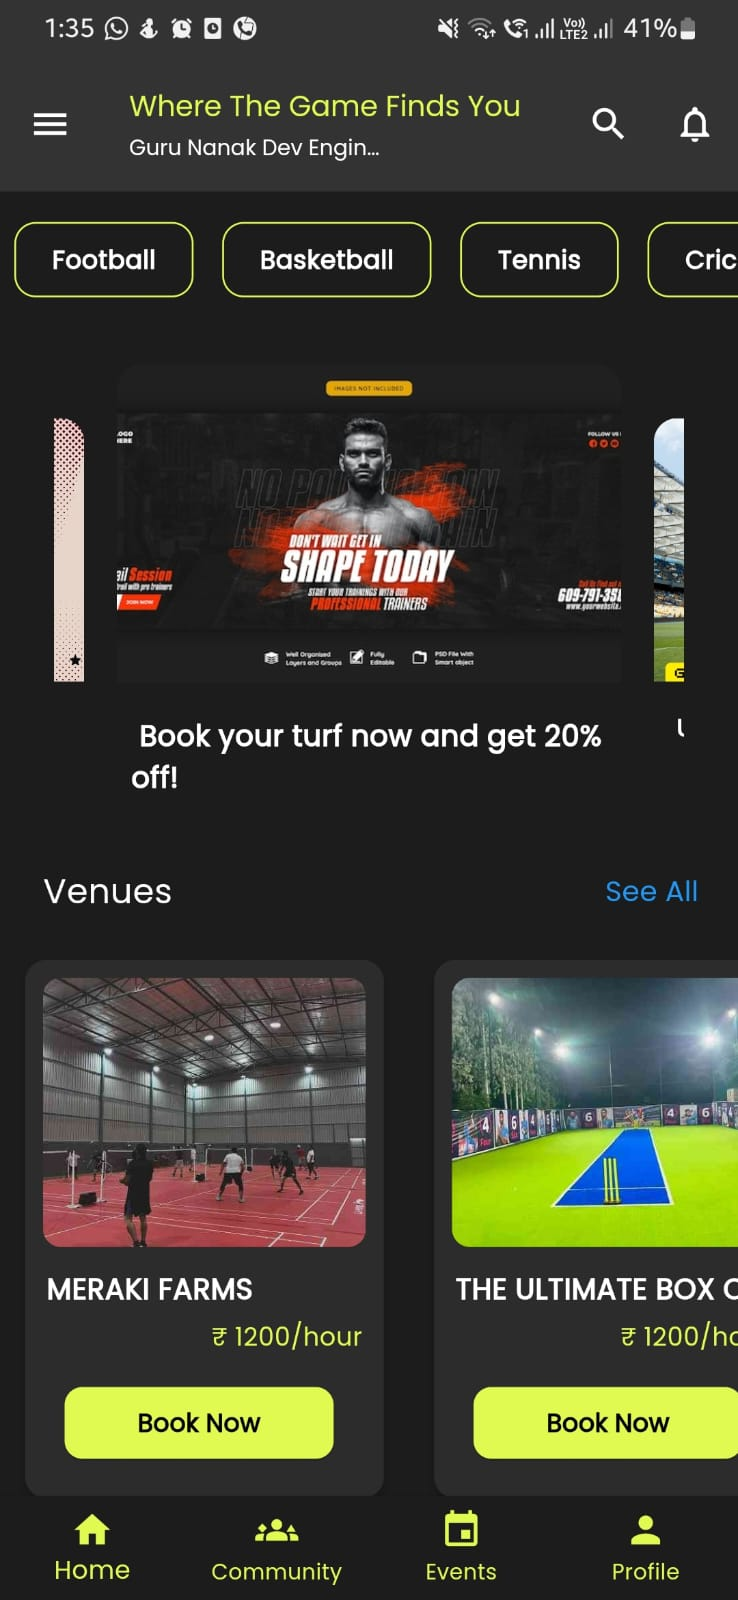
\includegraphics[width=0.9\textwidth]{assets/screenshot1.jpeg}
        \caption{Home Screen}
    \end{minipage}%
    \hfill
    \begin{minipage}[t]{0.3\textwidth}
        \centering
        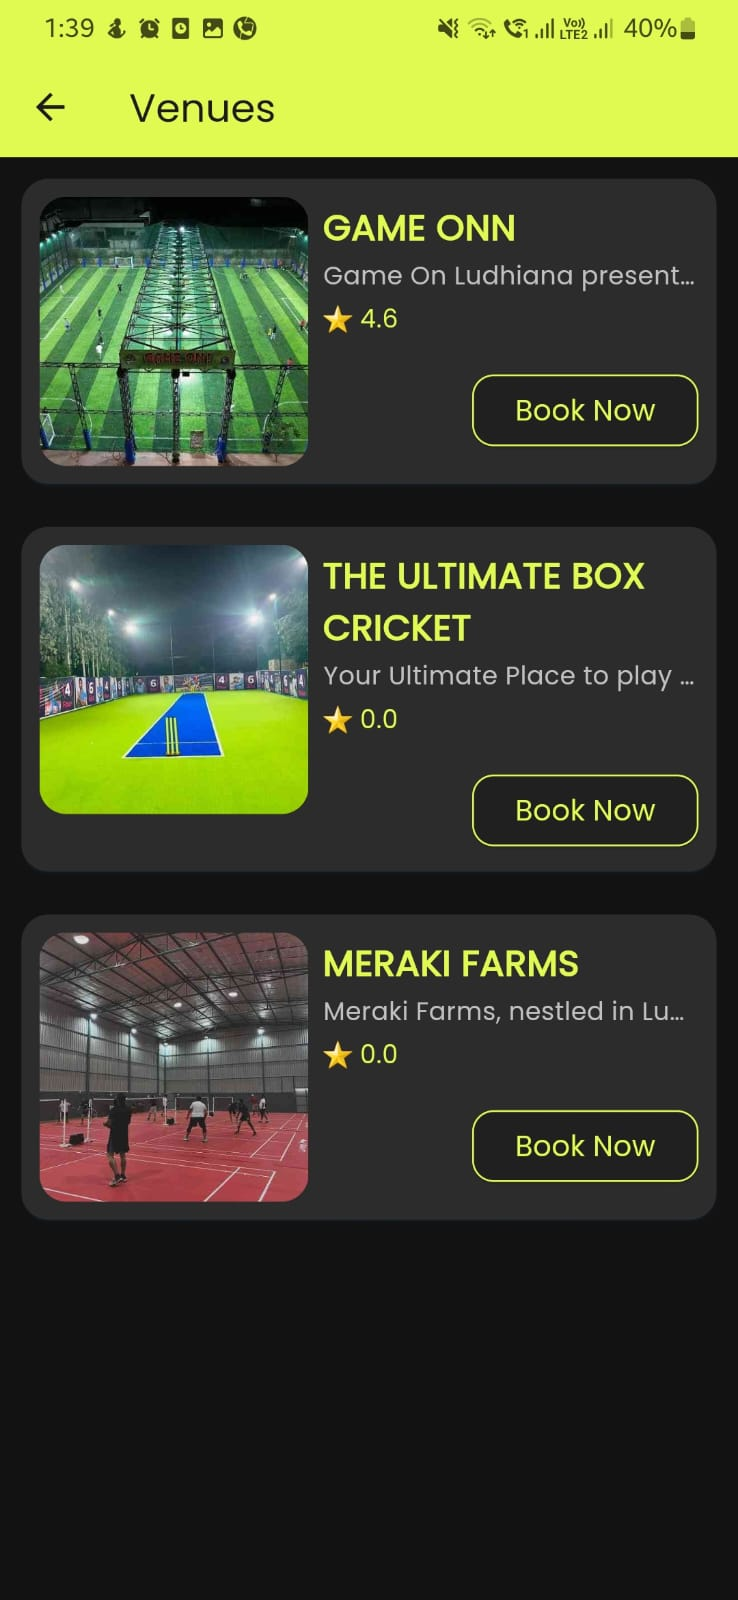
\includegraphics[width=0.9\textwidth]{assets/screenshot2.jpeg}
        \caption{All Venues}
    \end{minipage}
    \hfill
    \begin{minipage}[t]{0.3\textwidth}
        \centering
        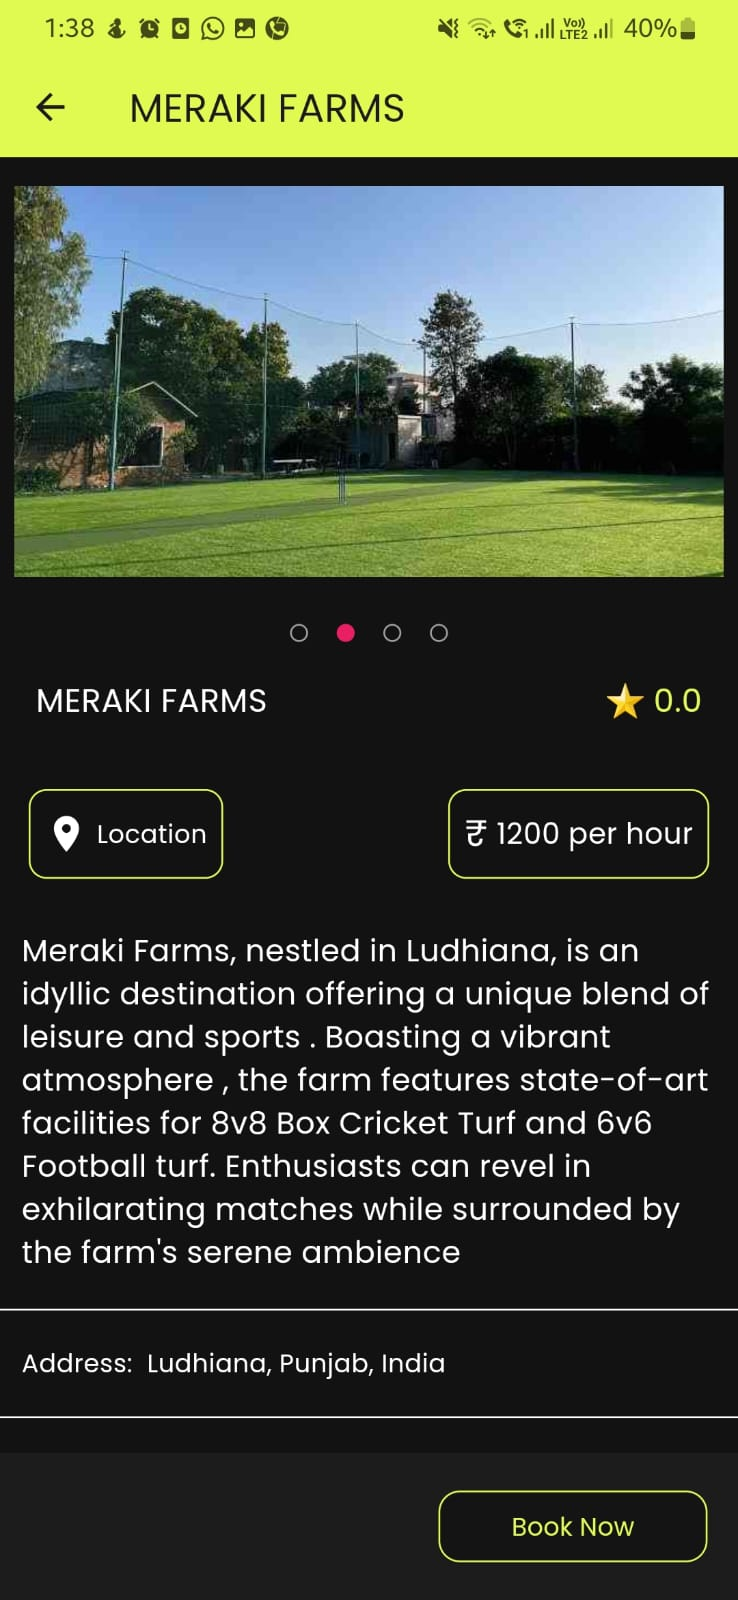
\includegraphics[width=0.9\textwidth]{assets/screenshot3.jpeg}
        \caption{Venue Detail}
    \end{minipage}

    \vspace{1cm}
    
    \begin{minipage}[t]{0.3\textwidth}
        \centering
        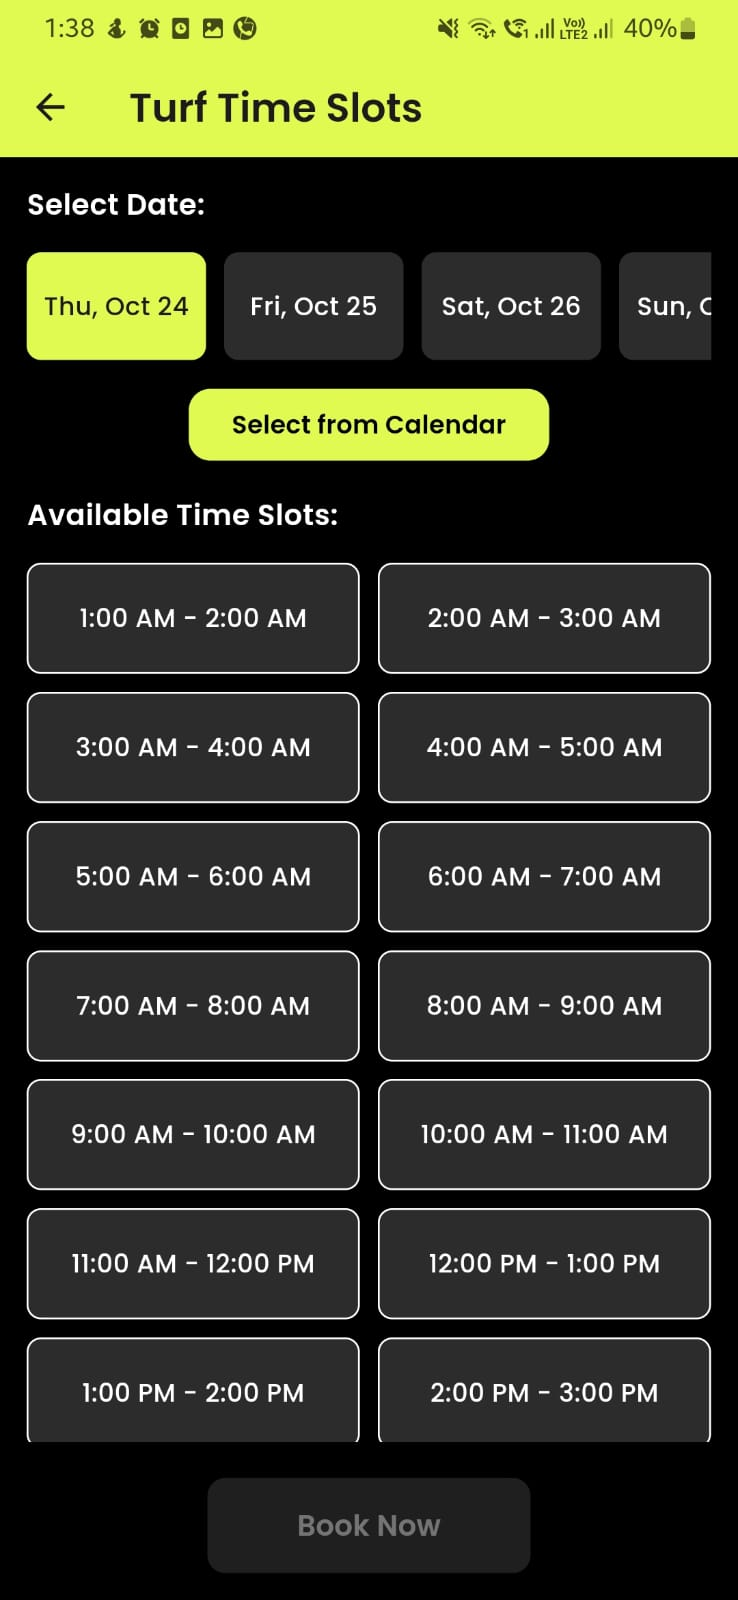
\includegraphics[width=0.9\textwidth]{assets/screenshot4.jpeg}
        \caption{Selecting Time Slots}
    \end{minipage}%
    \hfill
    \begin{minipage}[t]{0.3\textwidth}
        \centering
        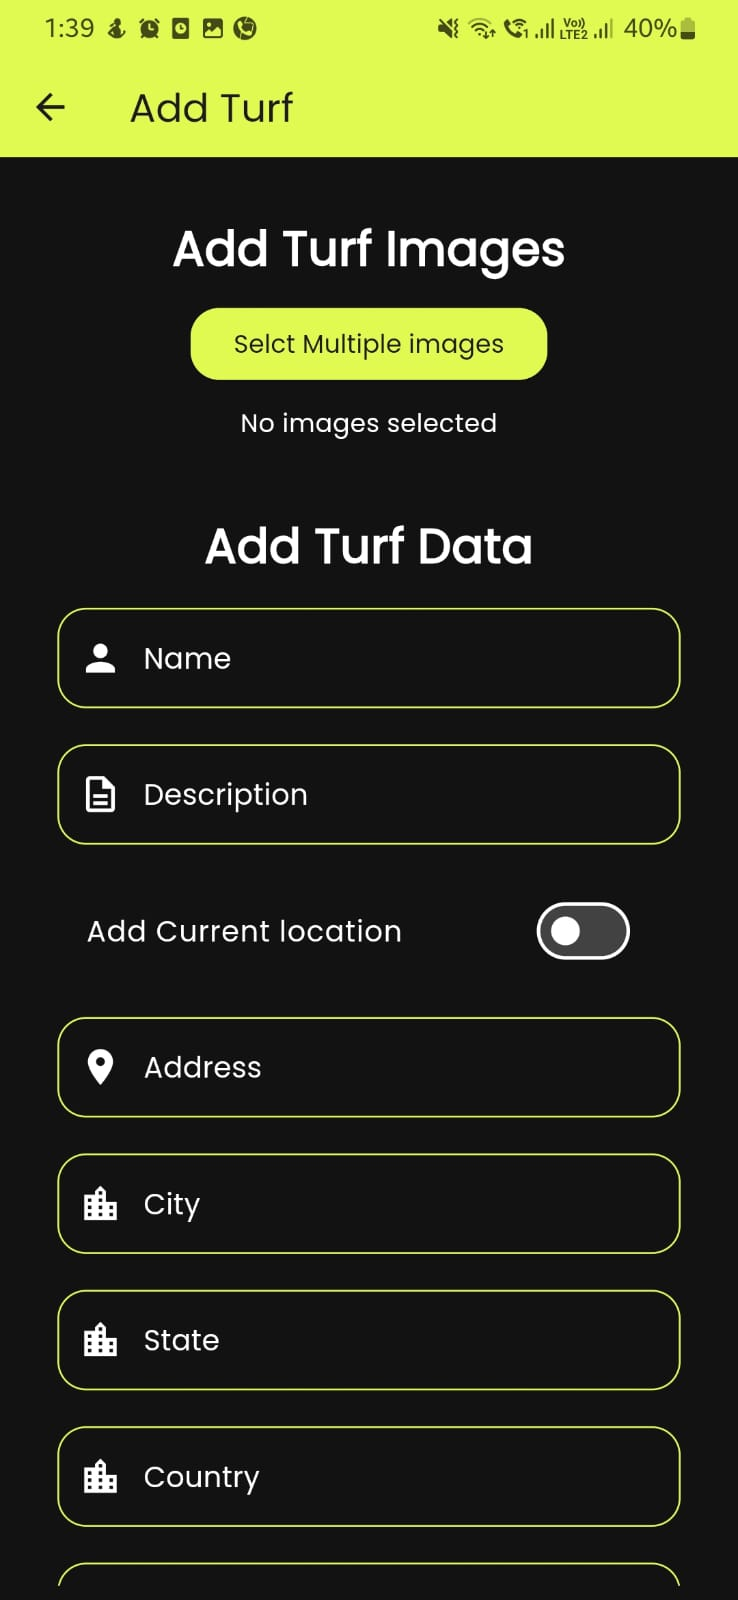
\includegraphics[width=0.9\textwidth]{assets/screenshot5.jpeg}
        \caption{Adding Venue}
    \end{minipage}
    \hfill
    \begin{minipage}[t]{0.3\textwidth}
        \centering
        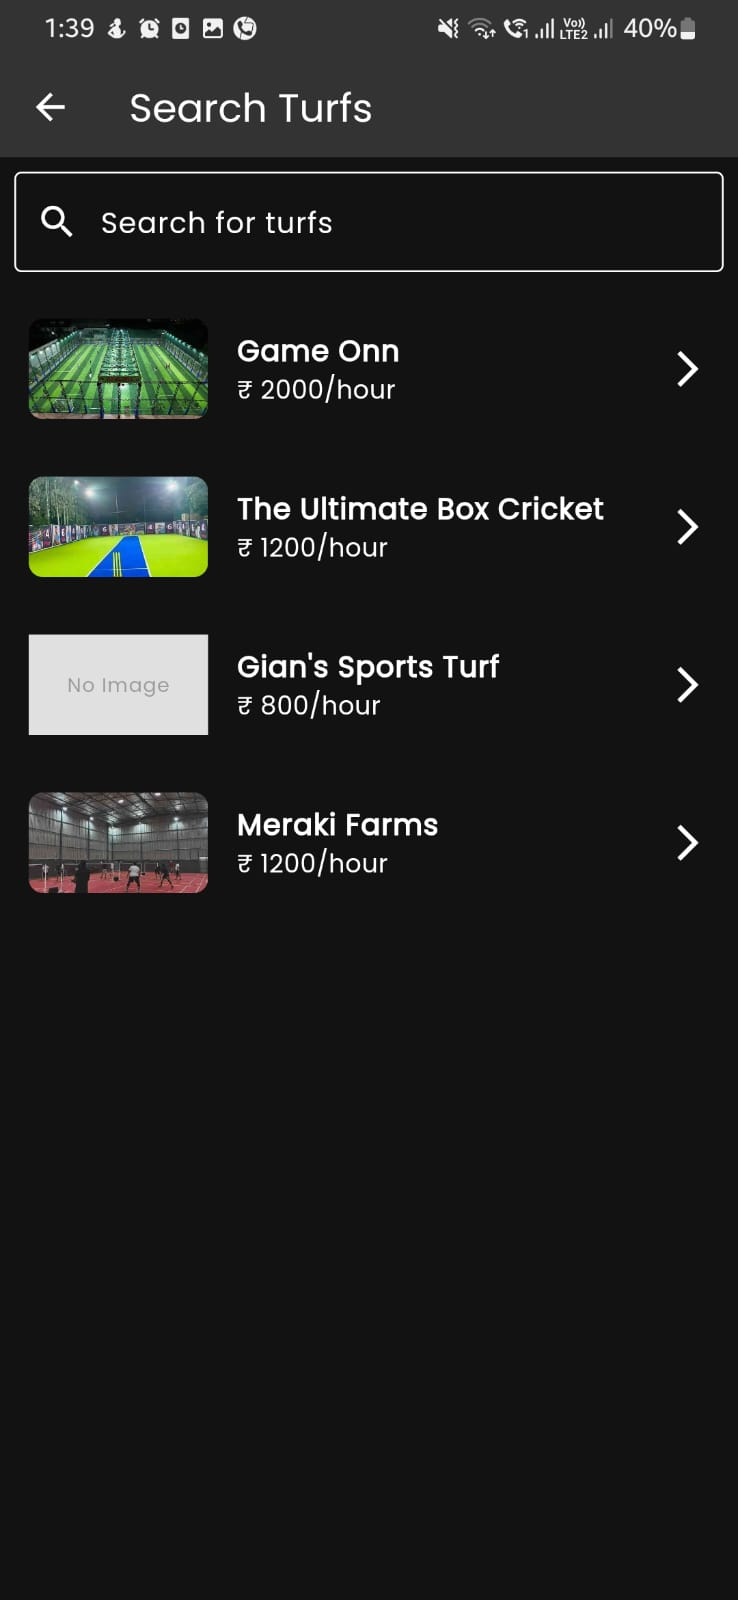
\includegraphics[width=0.9\textwidth]{assets/screenshot6.jpeg}
        \caption{Searching Venues}
    \end{minipage}
\end{figure}

\section{Future Enhancements}
While the current version of the SPOCO app serves its purpose, future enhancements could include:

\begin{itemize}
    \item \textbf{Payment Integration:} Implementing a secure payment gateway to facilitate online transactions for bookings.
    \item \textbf{Rating and Review System:} Allowing users to leave feedback on their experiences, improving the quality of services.
    \item \textbf{Push Notifications:} Integrating push notifications to keep users informed about booking reminders and new ground listings.
\end{itemize}

% Chapter 4: Conclusion and Future Scope
\chapter{Conclusion and Future Scope}

\section{Conclusion}
The development of the \textbf{SPOCO} app during my training in Mobile App Development using Flutter has been a transformative experience that significantly enhanced my skills and understanding of mobile application development. Under the guidance of \textbf{Auribises Technologies Pvt Ltd}, and with mentorship from \textbf{Ishank Kumar}, I gained hands-on experience in various aspects of app development, from foundational concepts in Dart to advanced Flutter functionalities.
Throughout the course, I acquired proficiency in key topics such as UI/UX design, state management, API integration, and Firebase backend services. These concepts were instrumental in shaping my approach to the SPOCO app, where I was responsible for implementing essential features such as user authentication, turf management, event creation, and booking processes. The collaborative nature of the project allowed me to work effectively with my peers, fostering teamwork and communication skills that are vital in the tech industry.
The \textbf{SPOCO} app effectively addresses the needs of users seeking to book sports grounds, demonstrating a user-friendly interface and streamlined booking process. The positive feedback received during testing highlighted the app's functionality and relevance, reinforcing the skills and knowledge I gained throughout my training.

\section{Future Scope}
While the S\textbf{Spoco} app is functional and meets its primary objectives, there are several areas for potential enhancement and future development that can further improve its overall functionality and user experience.

\subsection{Payment Gateway Integration}
One significant improvement would be the integration of a secure payment gateway. This feature would enable users to complete their bookings online, facilitating cashless transactions and enhancing convenience. Accepting various payment methods, such as credit/debit cards and digital wallets, would streamline the booking process and attract more users.

\subsection{Advanced User Features}
Although user profiles and community features are present in the SPOCO app, future enhancements could refine these functionalities:
\begin{itemize}
    \item \textbf{User Profile Customization:} Allowing users to personalize their profiles, manage preferences, and view booking history can enhance user engagement and retention.
    \item \textbf{Enhanced Community Interaction: } Developing features for users to connect, chat, or share experiences with others in the community can foster a sense of belonging and encourage user interaction.
\end{itemize}


\subsection{Enhanced Event Management}
Future updates could expand the event management capabilities by implementing:
\begin{itemize}
    \item \textbf{Event Notifications:}Sending timely notifications about upcoming events, new bookings, and changes to existing reservations would keep users informed and engaged.
    \item \textbf{User Feedback and Ratings: } Allowing users to leave feedback and rate their experiences can provide valuable insights for continuous improvement of the services offered.
\end{itemize}


\subsection{Multi-language Support}
Adding support for multiple languages would make the SPOCO app more inclusive, catering to a broader audience. This feature could significantly enhance the user experience for non-English speakers, thereby expanding the app's market reach.

\subsection{Marketing and Promotion Features}
Developing marketing tools within the app, such as promotional banners and discounts for early bookings, could attract more users and encourage frequent use of the platform. Collaborating with local sports organizations for promotions could also enhance visibility and user acquisition.


\section{Closing Thoughts}
In conclusion, the SPOCO app represents a significant achievement in my journey through the Mobile App Development course at Auribises Technologies. The knowledge and skills I have gained not only prepared me for real-world application development but also instilled in me a deeper appreciation for user-centric design and effective problem-solving. I look forward to applying the lessons learned from both the SPOCO project and the overall course in my future endeavors within the technology sector, continuing to innovate and create impactful mobile applications.


\end{document}
